\documentclass[border=20pt]{standalone}
\usepackage[american]{circuitikz}
\begin{document}
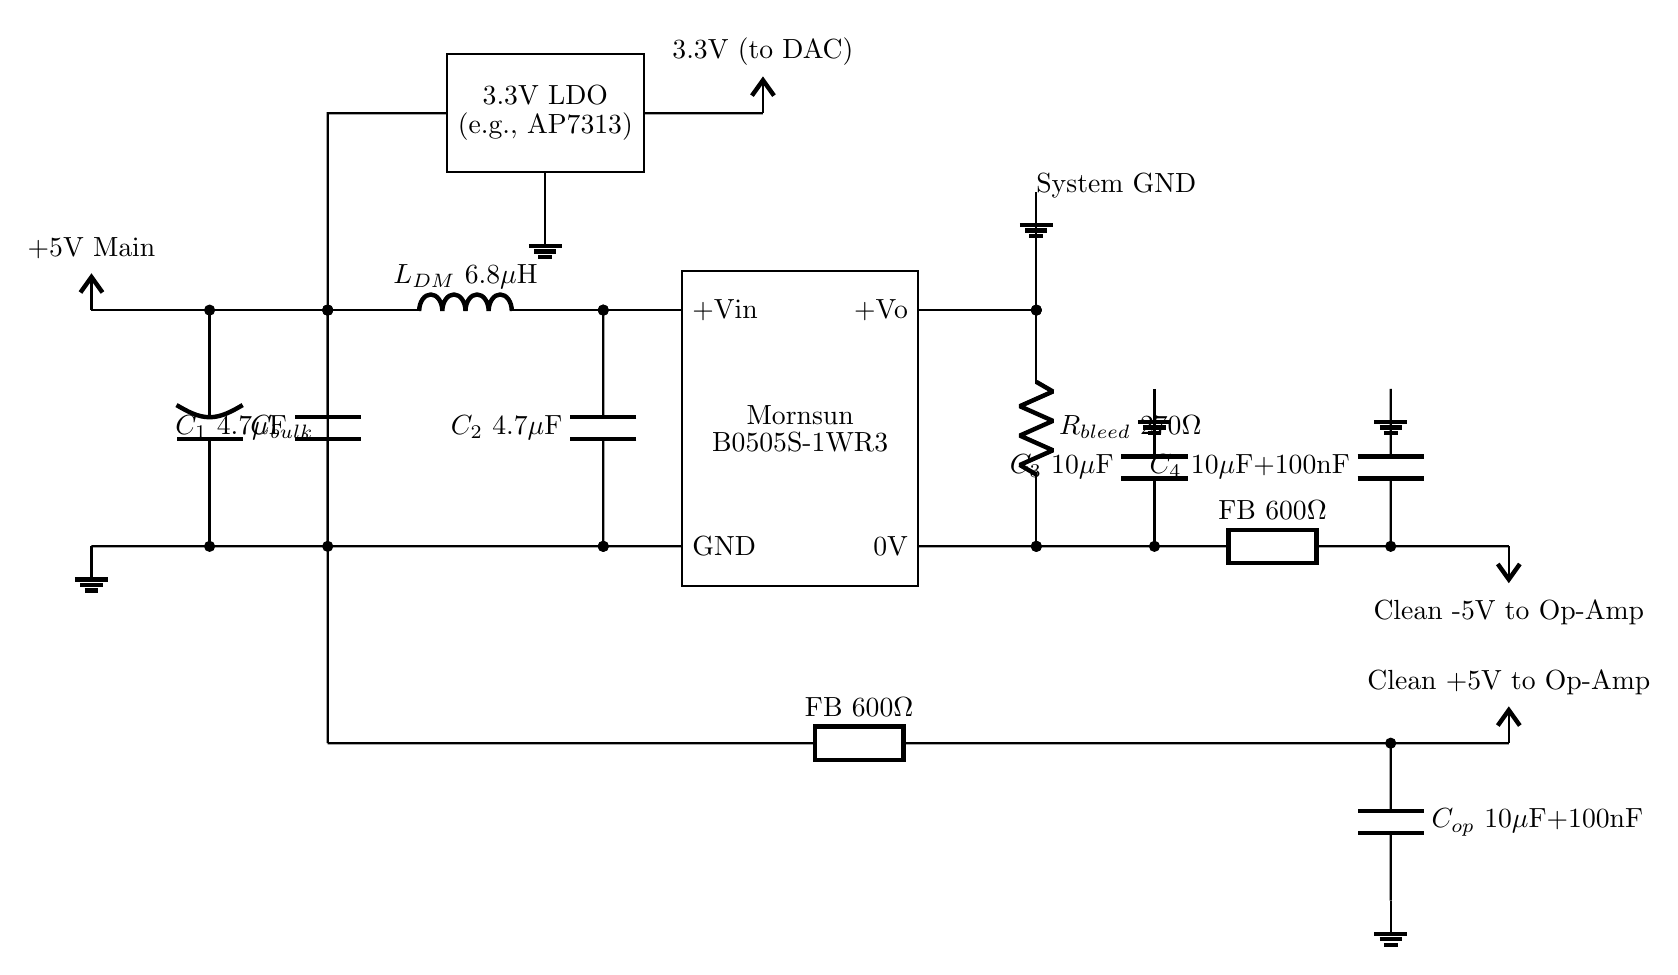
\begin{tikzpicture}[scale=1.0, transform shape, thick]

% Power Input
\node[vcc] (vcc_in) at (0,6) {+5V Main};
\node[ground] (gnd_in) at (0,3) {};

% Connect Input
\draw (vcc_in) to[short, -*] (1.5,6) coordinate (in_top);
\draw (gnd_in) to[short, -*] (1.5,3) coordinate (in_bot);
\draw (in_top) to[pC, l=$C_{bulk}$] (in_bot);

% Tap for LDO
\draw (in_top) to[short, -*] (3,6) coordinate (tap_ldo);
\draw (tap_ldo) to[short] (3,8.5) to[short] (4.5,8.5);
\node[draw, minimum width=2.5cm, minimum height=1.5cm, anchor=west] (ldo) at (4.5,8.5) {\shortstack{3.3V LDO\\(e.g., AP7313)}};
\draw (ldo.east) to[short] ++(1.5,0) node[vcc] {3.3V (to DAC)};
\draw (ldo.south) to[short] ++(0,-0.5) node[ground]{};

% Input Filter for DC-DC
\draw (tap_ldo) to[C, l_=$C_1$ $4.7\mu$F, *-*] (3,3);
\draw (3,3) to[short] (in_bot);

\draw (tap_ldo) to[L, l=$L_{DM}$ $6.8\mu$H, -*] (6.5,6) coordinate (dcdc_in);
\draw (3,3) to[short, -*] (6.5,3) coordinate (dcdc_gnd);
\draw (dcdc_in) to[C, l_=$C_2$ $4.7\mu$F, *-*] (dcdc_gnd);

% DC-DC Converter Box
\draw (7.5, 2.5) rectangle (10.5, 6.5);
\node at (9, 4.5) {\shortstack{Mornsun\\B0505S-1WR3}};
\node[anchor=west] at (7.5, 6) {+Vin};
\node[anchor=west] at (7.5, 3) {GND};
\node[anchor=east] at (10.5, 6) {+Vo};
\node[anchor=east] at (10.5, 3) {0V};

\draw (dcdc_in) to[short] (7.5, 6);
\draw (dcdc_gnd) to[short] (7.5, 3);

% Output side
\draw (10.5, 6) to[short, -*] (12, 6) coordinate (vo_plus);
\draw (10.5, 3) to[short, -*] (12, 3) coordinate (vo_minus);

% Grounding +Vo
\draw (vo_plus) to[short] (12, 7.5) node[ground]{System GND};

% Bleeder Resistor
\draw (vo_plus) to[R, l=$R_{bleed}$ $270\Omega$, *-*] (vo_minus);

% Pi Filter on -5V
\draw (vo_minus) to[short, -*] (13.5, 3) coordinate (pi1);
\draw (pi1) to[C, l=$C_3$ $10\mu$F] (13.5, 5) node[ground]{};
\draw (pi1) to[european resistor, l=FB $600\Omega$, -*] (16.5, 3) coordinate (pi2);
\draw (pi2) to[C, l=$C_4$ $10\mu$F+$100$nF] (16.5, 5) node[ground]{};
\draw (pi2) to[short] (18, 3) node[vee] {Clean -5V to Op-Amp};

% Clean 5V Tap for Op-Amp
\draw (tap_ldo) to[short, *-] (3, 0.5) coordinate (op_tap);
\draw (op_tap) to[european resistor, l=FB $600\Omega$, -*] (16.5, 0.5) coordinate (op_vcc);
\draw (op_vcc) to[C, l=$C_{op}$ $10\mu$F+$100$nF] (16.5, -1.5) node[ground]{};
\draw (op_vcc) to[short] (18, 0.5) node[vcc] {Clean +5V to Op-Amp};

\end{tikzpicture}
\end{document}
